\documentclass[a4paper]{article}
\usepackage[utf8x]{inputenc}
\usepackage[T1,T2A]{fontenc}
\usepackage[russian]{babel}
\usepackage{hyperref}
\usepackage{indentfirst}
\usepackage{listings}
\usepackage{color}
\usepackage{here}
\usepackage{array}
\usepackage{multirow}
\usepackage{graphicx}
\usepackage{amsmath} 
\usepackage{spverbatim}

\usepackage{caption}
\renewcommand{\lstlistingname}{Программа} % заголовок листингов кода

\lstset{ %
    extendedchars=\true,
    keepspaces=true,
    language=bash,					% choose the language of the code
    basicstyle=\footnotesize,		% the size of the fonts that are used for the code
    numbers=left,					% where to put the line-numbers
    numberstyle=\footnotesize,		% the size of the fonts that are used for the line-numbers
    stepnumber=1,					% the step between two line-numbers. If it is 1 each line will be numbered
    numbersep=5pt,					% how far the line-numbers are from the code
    backgroundcolor=\color{white},	% choose the background color. You must add \usepackage{color}
    showspaces=false				% show spaces adding particular underscores
    showstringspaces=false,			% underline spaces within strings
    showtabs=false,					% show tabs within strings adding particular underscores
    frame=single,           		% adds a frame around the code
    tabsize=2,						% sets default tabsize to 2 spaces
    captionpos=b,					% sets the caption-position to bottom
    breaklines=true,				% sets automatic line breaking
    breakatwhitespace=false,		% sets if automatic breaks should only happen at whitespace
    escapeinside={\%*}{*)},			% if you want to add a comment within your code
    postbreak=\raisebox{0ex}[0ex][0ex]{\ensuremath{\color{red}\hookrightarrow\space}}
}

\usepackage[left=2cm,right=2cm,
top=2cm,bottom=2cm,bindingoffset=0cm]{geometry}

\begin{document}	% начало документа

\begin{titlepage}	% начало титульной страницы

	\begin{center}		% выравнивание по центру

		\largeФедеральное государственное автономное образовательное учреждение высшего образования «Санкт-Петербургский политехнический университет Петра Великого» \\
		\large Институт компьютерных наук и технологий \\
		\large Кафедра компьютерных систем и программных технологий\\[2cm]
		% название института, затем отступ 6см
		
	    \vfill
		\hugeТелекоммуникационные технологии\\[0.5cm] % название работы, затем отступ 0,5см
		\large Лабораторная работа №1,2:\\
		"Сигналы телекомуникационных систем.\\ Ряд Фурье. Преобразование Фурье. Корреляция"\\[4.8cm]

	\end{center}

	\begin{flushright} % выравнивание по правому краю
		\begin{minipage}{0.25\textwidth} % врезка в половину ширины текста
			\begin{flushleft} % выровнять её содержимое по левому краю

				\large\textbf{Работу выполнил:}\\
				\large Сергеев ~А.А.\\
				\large {Группа:} 33531/2\\
				
				\large \textbf{Преподаватель:}\\
				\large Богач ~Н.В.\\

			\end{flushleft}
		\end{minipage}
	\end{flushright}
	
	\vfill % заполнить всё доступное ниже пространство

	\begin{center}
	\large Санкт-Петербург\\
	\large \the\year % вывести дату
	\end{center} % закончить выравнивание по центру

\thispagestyle{empty} % не нумеровать страницу
\end{titlepage} % конец титульной страницы
\vfill % заполнить всё доступное ниже пространство


% Содержание
\tableofcontents
\newpage
\section{Цель работы}
Получить представление о спектрах телекоммуникационных сигналов.
\section{Постановка задачи}
\begin{enumerate}
    \item Для сигналов, построенных в лабораторной работе № 1, выполните расчет преобразования Фурье. Перечислите свойства преобразования Фурье.
    \item С помощью функции корреляции найдите позицию синхропосылки [101] в сигнале [0001010111000010]. Получите пакет данных, если известно, что его длина составляет 8 бит без учета синхропосылки. Вычислите корреляцию прямым методом, воспользуйтесь алгоритмом быстрой корреляции, сравните время работы обоих алгоритмов.
    \item Быстрая корреляция
\end{enumerate}
\section{Теоретический раздел}
\subsection{Сигнал. Виды сигналов}
Сигнал -- это функция, несущая сообщение (данные) о физических свойствах, состоянии или поведении какой-либо физической системы, объекта или среды.\\
Спектр сигнала -- это результат разложения сигнала на более простые в базисе ортогональных функций. В качестве разложения обычно используются преобразование Фурье и другие.\\
Виды сигналов:
\begin{enumerate}
    \item Аналоговый сигнал
    \item Дискретный сигнал
    \item Цифровой сигнал
\end{enumerate}
Сигналы можно классифицировать:
\begin{enumerate}
    \item По точности:
    \begin{itemize}
        \itemдетерминированные: сигнал полностью известен
        \itemслучайные: в любой момент времени сигнал представляет собой случайную величину
    \end{itemize}
    \item Сигнал с интегрируемым квадратом $\int_{-\infty}^{+\infty}s^2(t)dt<\infty$
    \item По периодичности:
    \begin{itemize}
        \item сигналы с периодом T
        \item непериодичные
    \end{itemize}
    \item Сигналы конечной длительности (отличны от нуля только на ограниченном промежутке времени)
    \item Тестовые:
    \begin{itemize}
    \itemгармонические: $s(t)=A\cos{(\omega t+ \phi)}$
    \itemфункция Дирака: дельта-функция $\delta(t)$
    \itemфункция Хевисайда: функция единичного скачка $\sigma(t)$
    \end{itemize}
\end{enumerate}
Анализ -- это один из ключевых компонентов обработки сигналов. Основной целью анализа определяют сравнение сигналов друг с другом для определения их сходств и различий. \\
Выделяют три основные составляющие анализа сигналов:
\begin{enumerate}
    \item измерение числовых параметров сигналов
    \item разложение сигнала на элементарные составляющие
    \item количественное измерение степени <<похожести>> различных сигналов
\end{enumerate}
\subsection{Ряд Фурье. Преобразование Фурье}
Ряд Фурье — представление произвольной функции $f$ с периодом $\tau$ в виде ряда: $$f(x)=\frac{a_0}{2}+\sum_{k=1}^{+\infty}A_k\cos{(2\pi\frac{k}{\tau}x+\theta_k)}$$. Этот ряд может быть также записан в виде $f(x)=\sum_{k=1}^{+\infty}\widehat{f}_k e^{i2\pi\frac{k}{\tau}x}$,\\
где $A_k$ -- амплитуда $k$-го гармонического колебания,\\
$2\pi\frac{k}{\tau}=k\omega$ -- круговая частота гармонического колебания,\\
$\theta_k$ -- начальная фаза $k$-го колебания,\\
$\widehat{f}_k$ -- $k$-я комплексная амплитуда.\\
Разложение функции в ряд Фурье является мощным инструментом при решении самых разных задач благодаря тому, что ряд Фурье прозрачным образом ведёт себя при дифференцировании, интегрировании, сдвиге функции по аргументу и свёртке функций.\\
Тригонометрическим рядом Фурье функции $f\in L_2([-\pi, \pi])$ называют функциональный ряд вида $$f(x)=\frac{a_0}{2}+\sum_{n=1}^{\infty}(a_n\cos{nx}+b_n\sin{nx})$$
где $a_0=\frac{1}{\pi}\int_{-\pi}^{\pi}f(x)dx$,\\
$a_n=\frac{1}{\pi}\int_{-\pi}^{\pi}f(x)\cos{nx}dx$,\\
$b_n=\frac{1}{\pi}\int_{-\pi}^{\pi}f(x)\sin{nx}dx$,\\
числа $a_0, a_n, b_n (n=1,2,...)$ называются коэффициентами Фурье функции $f$.\\
Определим прямое и обратное преобразование Фурье:\\
прямое $\widehat{f}(\omega)=\int_{-\infty}^{+\infty}f(x)e^{-2x\pi i}dx$\\
обратное $\widehat{f}(x)=\int_{-\infty}^{+\infty}f(\omega)e^{2x\pi i}d\omega$\\
С помощью обратного преобразования можно получить изначальный сигнал, то есть до и после -- взаимозаменяемы и несут одну и ту же информацию. Однако потеря участка начального сигнала во времени может внести сильные изменения в спектр, в то время как потеря информации о некоторых частотах может быть не так значительна.
\subsection{Свойства преобразования Фурье}
Рассмотрим сигналы: $f(t)$ и $g(t)$. Их спектральные функции: $\dot{F}(\omega)$ и $\dot{G}(\omega)$ соответственно.\\
\begin{itemize}
\item Линейность: линейная комбинация преобразованных равна результату преобразования линейных
комбинаций.
Если $s(t)=\alpha f(t)+\beta g(t)$, то $\dot{S}(\omega)=\alpha\dot{F}(t)+\beta\dot{G}(t)$\\
\item Задержка сигнала: можно двигать сигнал по оси времени, это изменит его фазовый спектр на известную величину $\tau$.\\
Если $s(t)=f(t-\tau)$, то $\dot{S}(\omega)=\dot{F}(\omega)e^{-j\omega\tau}$.\\
\item Масштабирование: спектр исходной функции изменяется в ширине обратно пропорционально сигналу.\\
Если $s(t)=f(\alpha t)$,то $\dot{S}(\omega)=\frac{1}{|\alpha|}\dot{F}(\alpha)$, $\alpha\neq0$.\\
\item Спектр свертки: произведение спектров может сказать о том, как система воздействует на сигнал.\\
$$\dot{S}(\omega)=\dot{F}(\omega)\dot{G}(\omega)$$
\item Умножение сигнала на гармоническую функцию: в итоге имеем слагаемые уменьшенной амплитуды, разнесенных на частоту гармоники в разные стороны от начального спектра. Если мы хотим отрезать какую-то часть частот, это удобно использовать.\\
$s(t)=f(t)\cos{(\omega_0t+\phi_0)}$\\
\item Спектр сигнала: в радиотехнике это результат разложения сигнала на более простые в базисе ортогональных функций. В качестве разложения обычно используем преобразование Фурье.\\
$\dot{S}(\omega)=\frac{1}{2}e^{i\phi_0}\dot{F}(\omega-\omega_0)+\frac{1}{2}e^{-i\phi_0}\dot{F}(\omega+\omega_0)$\\
\end{itemize}
\subsection{Корреляция сигналов}
Корреляция применяется для измерения степени схожести двух сигналов. Взаимная корреляция:
$$r_{12}(i)=\frac{1}{N}\sum_{n=0}^{N-1}x_2(n)x_1(n+i)$$
где $n$ -- временные отсчеты, $i$ -- задержка (число отсчетов, на которые сигнал $x_2$ отстает от сигнала $x_1$). Для непрерывных сигналов с периодом $T$ функция взаимной корреляции определяется следующим
образом:
$$r_{12}(\tau)=\frac{1}{T}\int_{0}^{T}x_1(t)x_2(\tau+t)dt$$
Для сигналов конечной длительности:
$$r_{12}(\tau)=\frac{1}{T}\int_{-\infty}^{+\infty}x_1(t)x_2(\tau+t)dt$$
Теорема о корреляции:
$$r_{12}=\frac{1}{N}F^{-1}_D[\overline{X}_1(k)X_2(k)]$$
где $X_1(k)=F_D[x_1(n)]$, $X_2(k)=F_D[x_2(n)]$, $F_D$ и $F_D^{-1}$ -- прямое и обратное ДПФ, которые вычисляются с использованием алгоритма БПФ.\\
Если число элементов в последовательностях $x_1(n)$ и $x_2(n)$ достаточно велико, то быстрой корреляцией
ответ будет получен быстрее, чем при расчете с помощью взаимной корреляции.
\section{Ход работы}
\subsection{Сигналы и их спектры}
\subsubsection{Синусоидальный сигнал. Спектр синусоидального сигнала}
\lstinputlisting[language=Matlab]{lab1/signals/sin_sig.m}\\
Синусоидальный сигнал\\
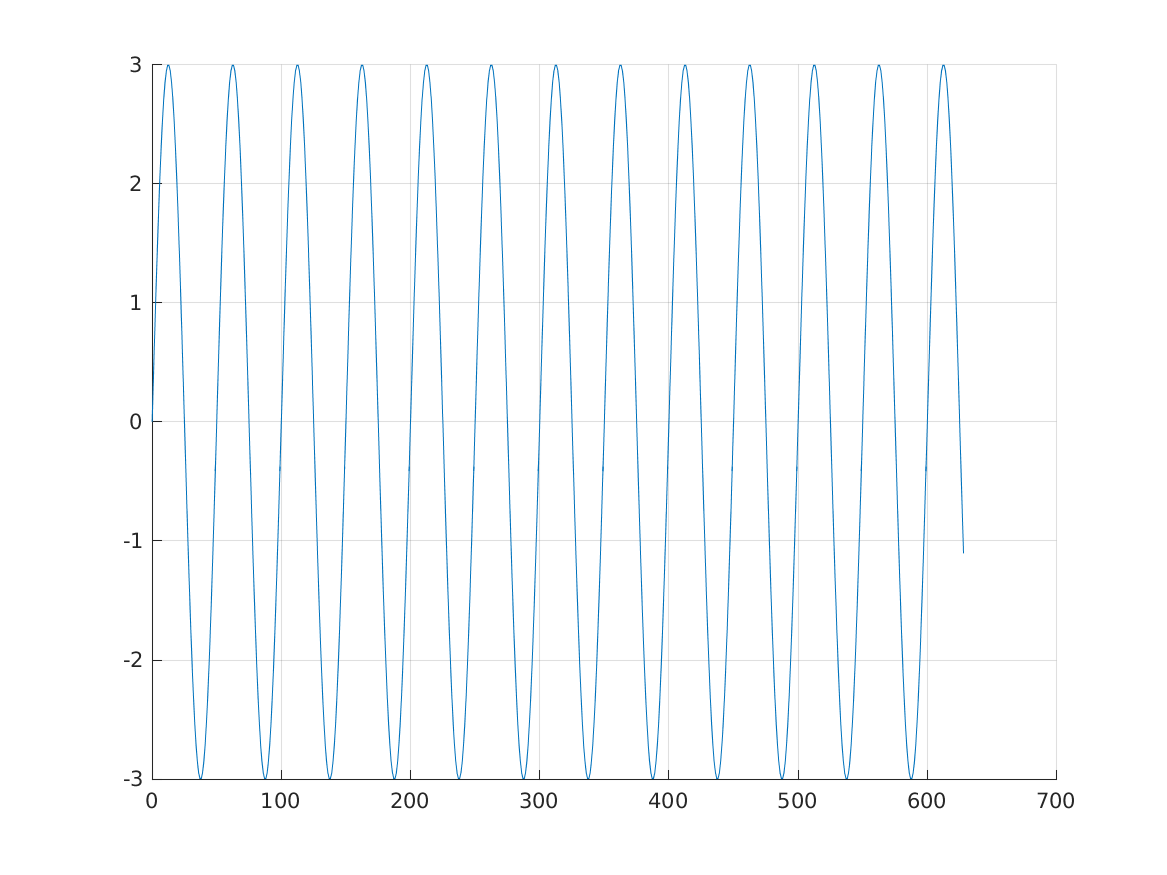
\includegraphics[scale=0.7]{figures/figure_0.png}\\
Спектр синусоидального сигнала\\
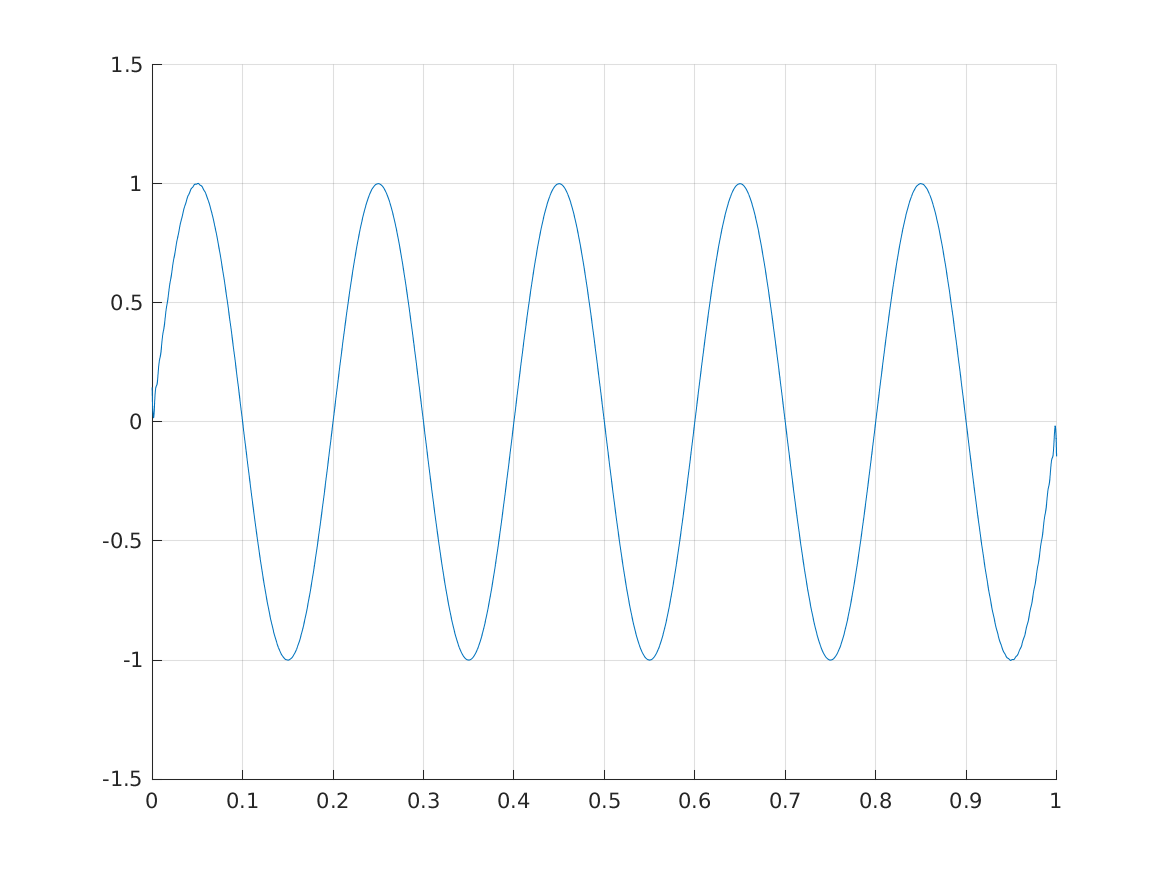
\includegraphics[scale=0.7]{figures/figure_2.png}
\newpage
\subsubsection{Прямоугольный сигнал. Спектр прямоугольного сигнала}
\lstinputlisting[language=Matlab]{lab1/signals/square_sig.m}\\
Прямоугольный сигнал\\
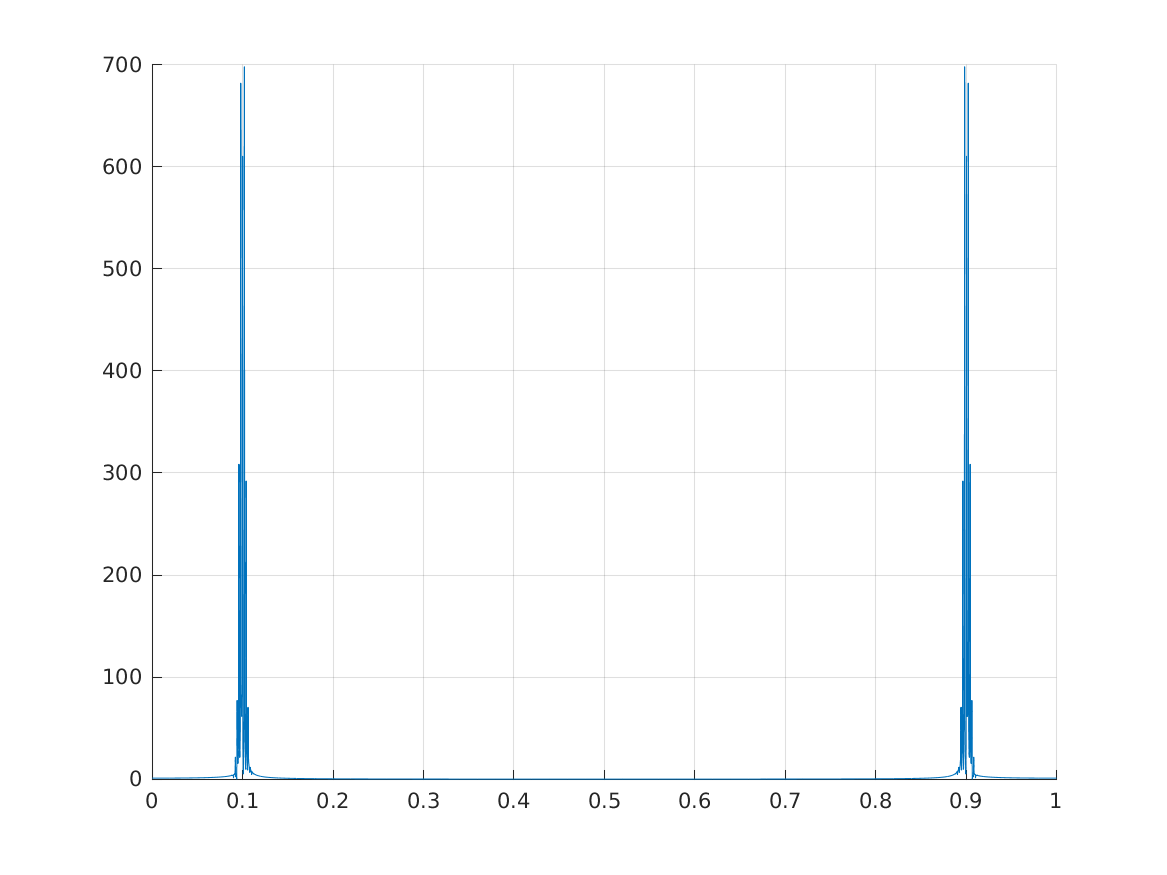
\includegraphics[scale=0.7]{figures/figure_3.png}\\
Спектр прямоугольного сигнала\\
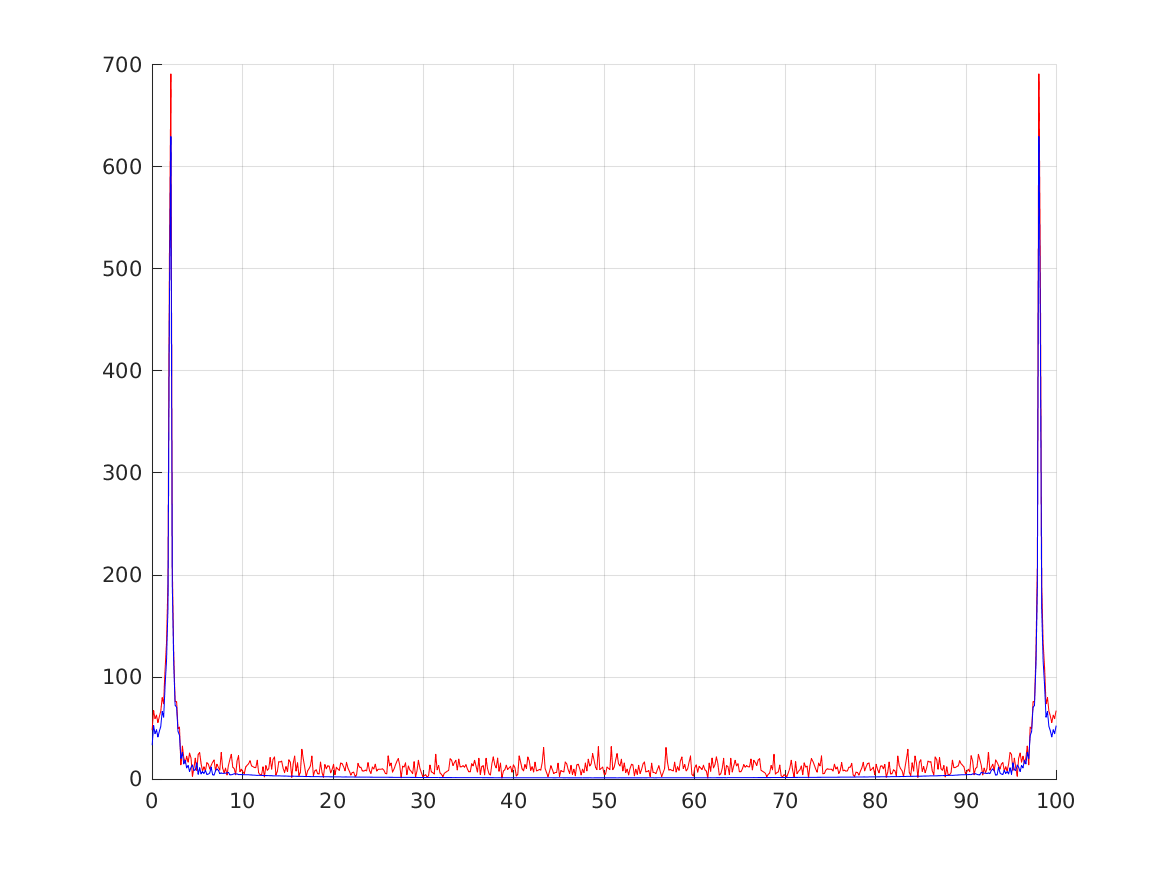
\includegraphics[scale=0.7]{figures/figure_5.png}
\subsubsection{Треугольный сигнал. Спектр треугольного сигнала}
\lstinputlisting[language=Matlab]{lab1/signals/triangle_sig.m}\\
Треугольный сигнал\\
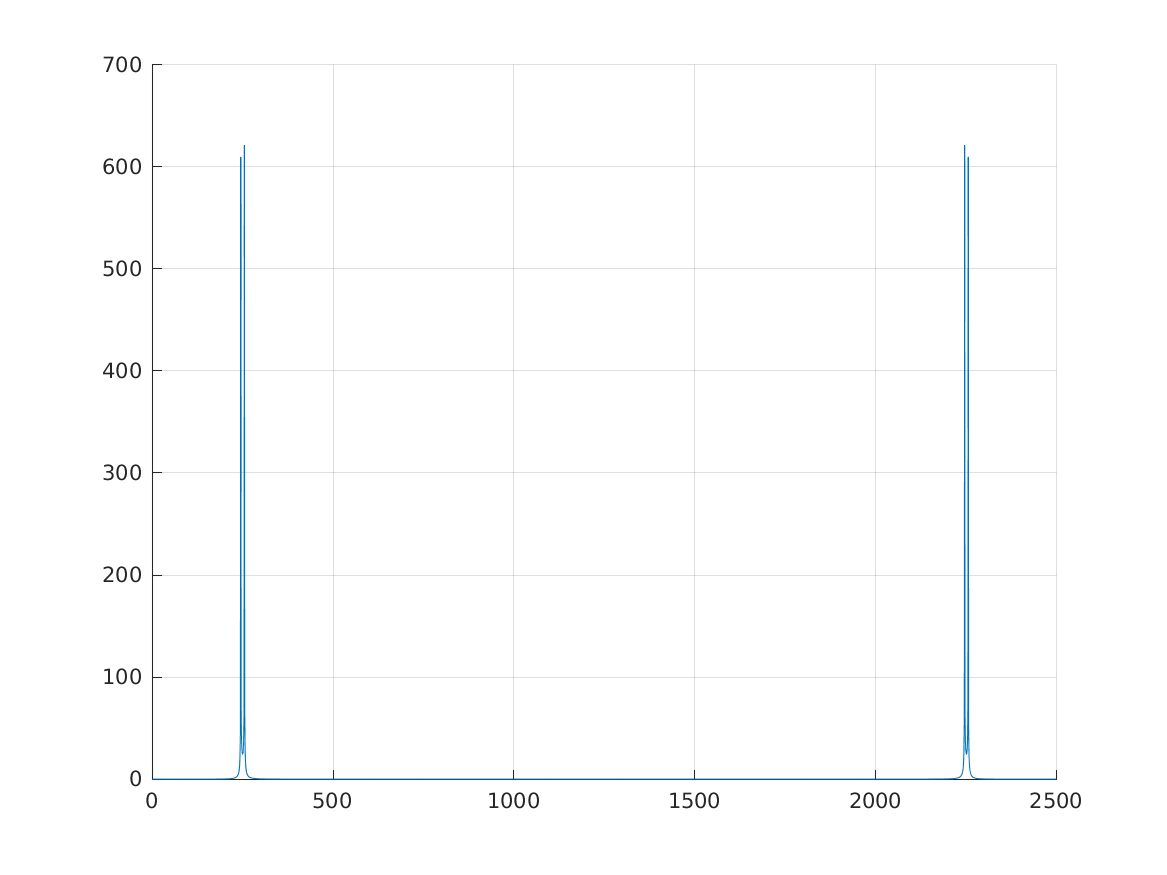
\includegraphics[scale=0.7]{figures/figure_6.png}\\
Спектр треугольного сигнала\\
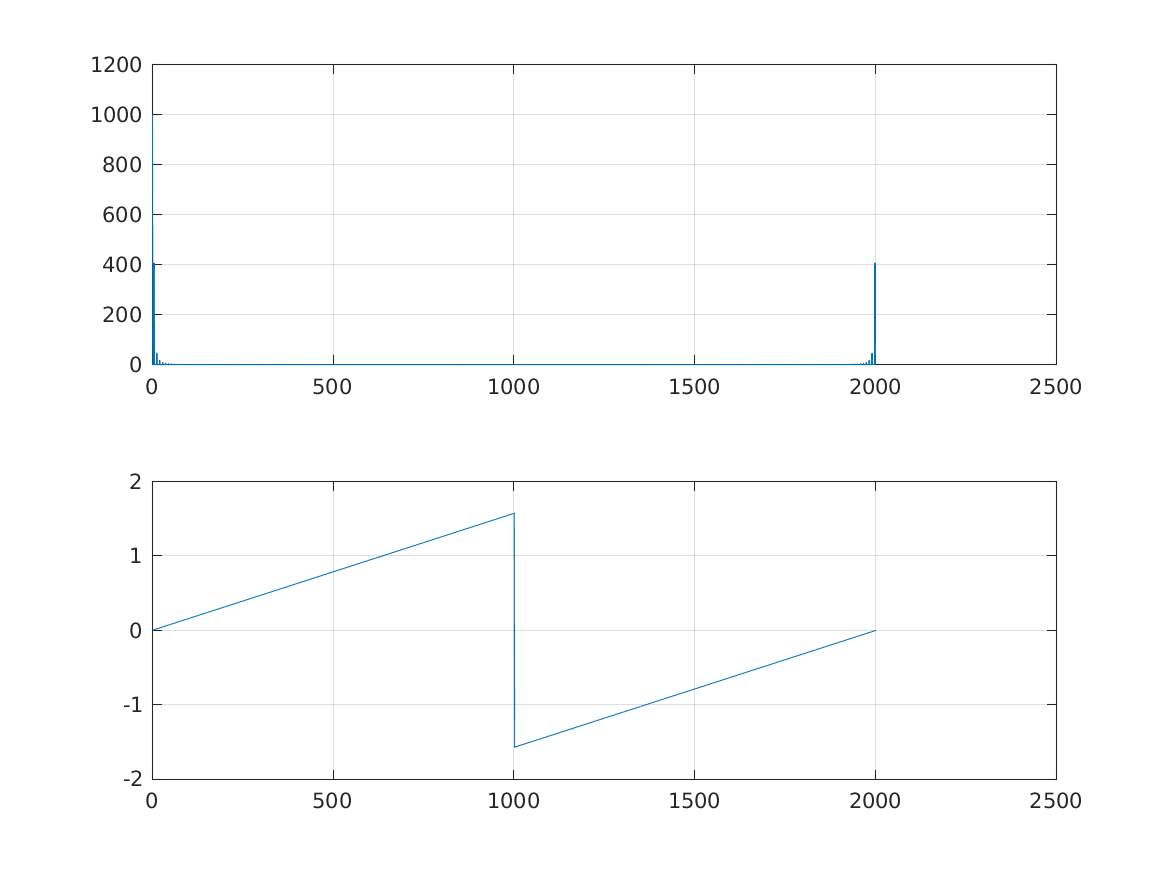
\includegraphics[scale=0.7]{figures/figure_8.png}
\subsection{Преобразования Фурье для сигналов}
Зададим различные сигналы так же, как делали это в лабораторной работе 1. Затем посмотрим их спектры.
Формирование сигналов происходит по тому же принципу что в лабораторной работе 1.
Затем получим преобразование Фурье для всех заданных сигналов и построим графики самих функций, амплитудные спектры и фазовые:\\
\newpage
\lstinputlisting[language=Matlab]{lib/matlab/draw/draw_spectrums.m}\\
\\
\subsubsection{Синусоидальный сигнал}
Амплитудный и фазовый спектры синусоидального сигнала:\\
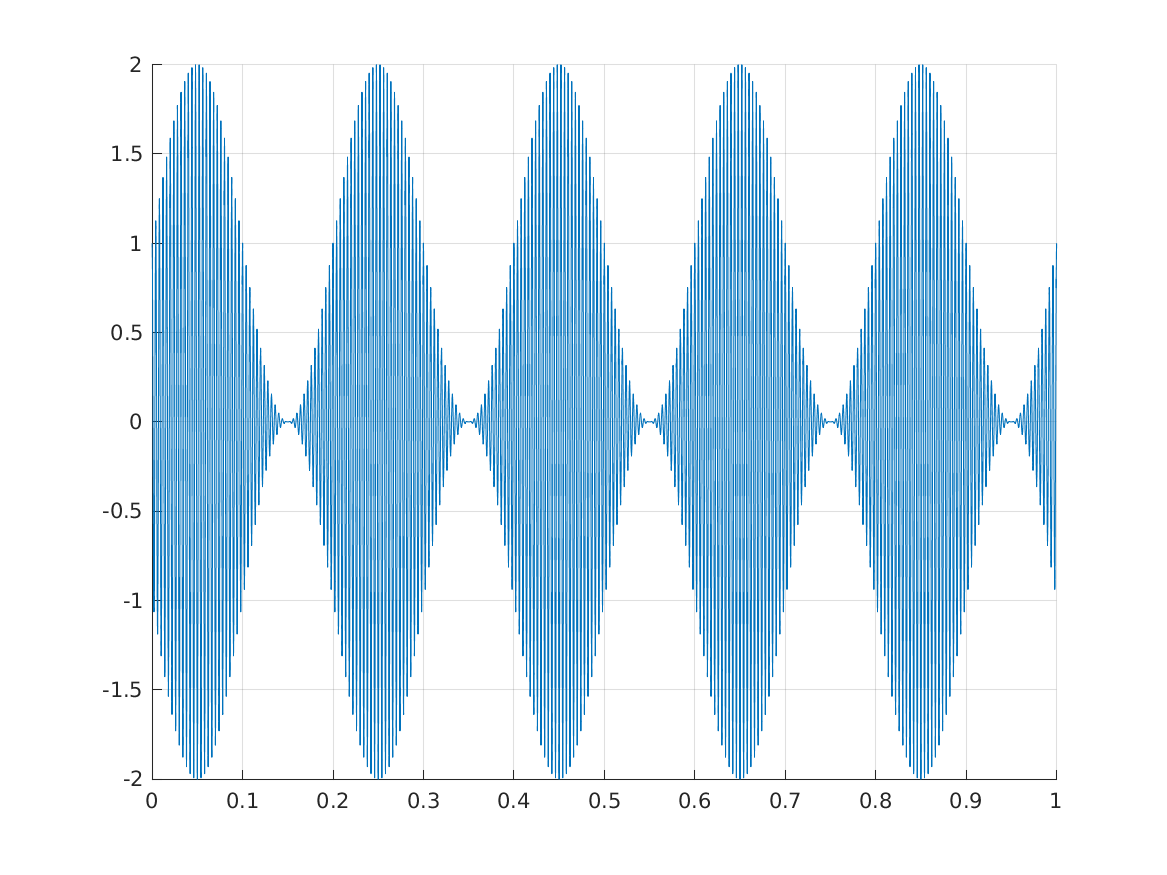
\includegraphics[scale=0.7]{figures/figure_1.png}
\subsubsection{Прямоугольный сигнал}
Амплитудный и фазовый спектры прямоугольного сигнала:\\
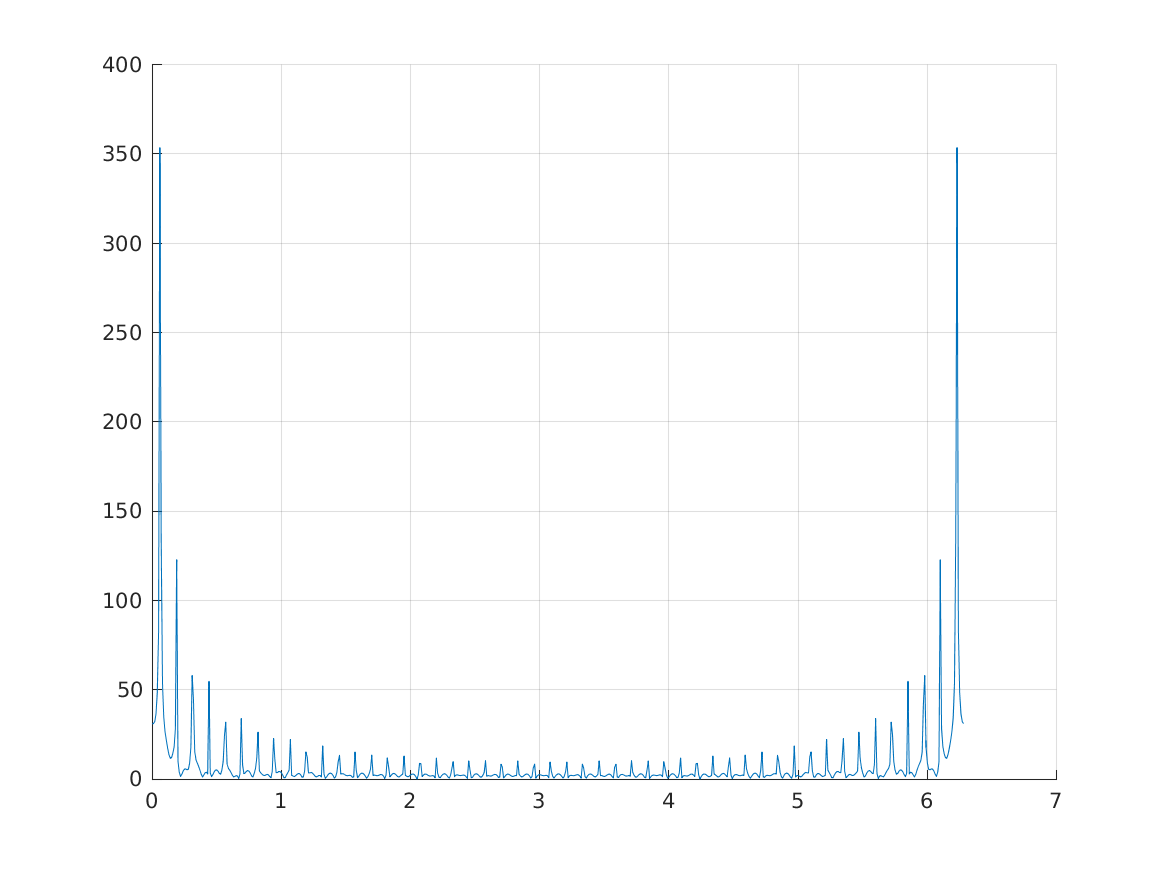
\includegraphics[scale=0.7]{figures/figure_4.png}\\
\subsubsection{Треугольный сигнал}
Амплитудный и фазовый спектры треугольного сигнала:\\
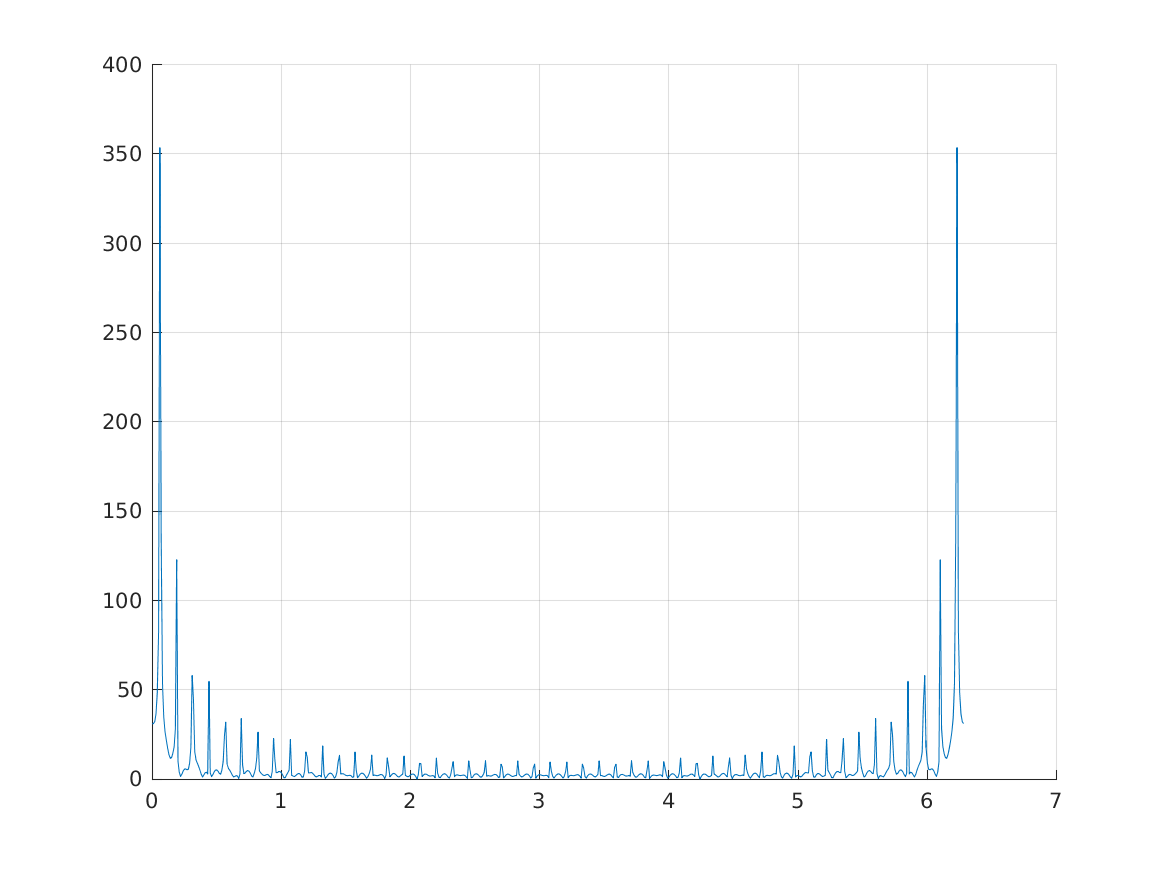
\includegraphics[scale=0.7]{figures/figure_7.png}\\
\subsection{Корреляция прямым методом и быстрая корреляция}
Сравним время вычисления с помощью обычной корреляции ($xcorr$) и быстрой корреляции (см. формулу в теор. разделе).\\
\lstinputlisting[language=Matlab]{lab1/correlations/normal_correlation.m}\\
\lstinputlisting[language=Matlab]{lab1/correlations/fast_correlation.m}\\
Обычная корреляция:\\
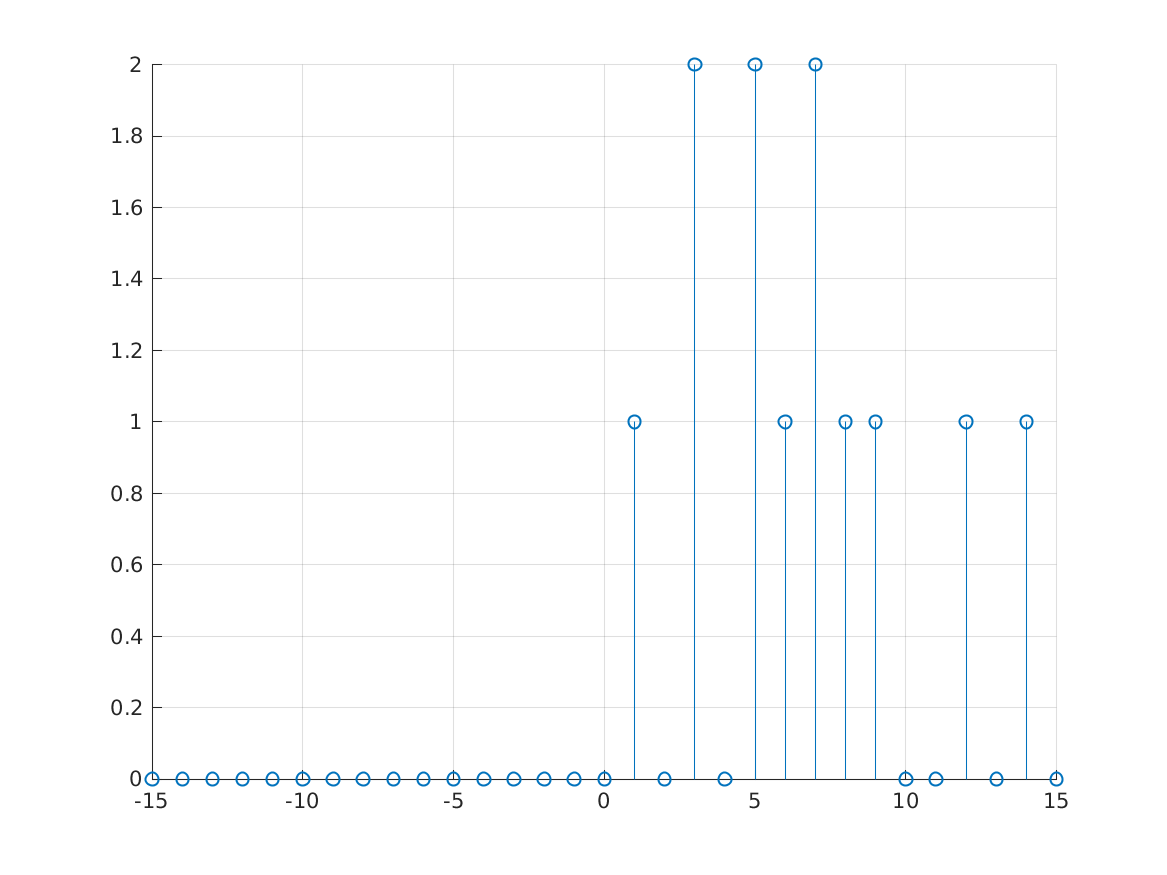
\includegraphics[scale=0.4]{figures/figure_9.png}\\
Быстрая корреляция:\\
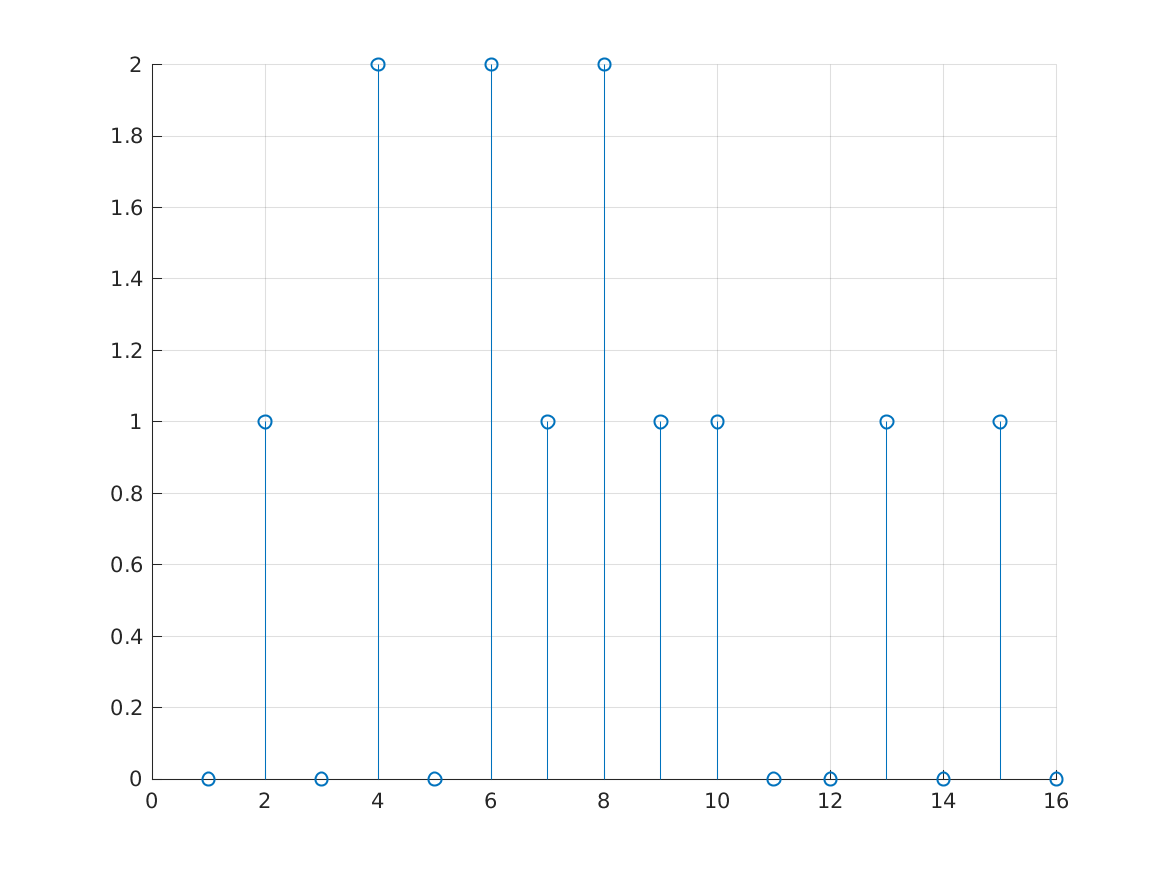
\includegraphics[scale=0.4]{figures/figure_10.png}\\
Время вычисления обычной корреляции $0.2245$, быстрой -- $0.0069$.\\
\newpage
\section{Вывод}
В результате работы , были промоделированы синусоидальный, прямоугольный и треугольный сигналы
В зависимости от известных параметров и требований сигналы подразделяются на группы:
\begin{enumerate}
    \item Если сигнал известен полностью, то он является детерминированным.
    \item Если в любой момент времени сигнал представляет собой случайную величину, то он называется случайным.
    \item Сигналы, у которых есть период, являются периодическими.
\end{enumerate}
Преобразование Фурье нашло широкое применение в телекоммуникационных технологиях. При исследовании сигналов его использование позволяет совершать переход из временной области в частотную и наоборот. Рассматривая сигналы во времени, мы не всегда можем определить все необходимые нам их характеристики. В то время как их частотное представление позволяет идентифицировать недостающий ряд параметров.\\
Так же были исследованы функции корреляции прямым и быстрым методами, и была найдена позиция синхропосылки в сигнале.
\end{document}